% SC3270 --- Chapter 4: Verifying Loops - Putting Invariants to Work (0->100 ground-up)
\chapter{Verifying Loops: Putting Invariants to Work}
\label{ch:loop-verify}

\begin{quote}
\emph{``A loop without an invariant is a story without a thesis: it may be entertaining, but you cannot tell whether it ends correctly.''} This chapter turns invariants into complete proofs and verification conditions.
\end{quote}

\noindent\fbox{\parbox{\dimexpr\linewidth-2\fboxsep-2\fboxrule}{%
\textbf{From zero: loop proofs built from first principles.} We assume only the invariant idea from Chapter~3 and build the full Hoare while-rule, generate VCs mechanically, and verify classic loops end-to-end. No prior VC experience needed.}}
\vspace{0.4em}

\section*{Learning Outcomes}
After this chapter you will be able to:
\begin{enumerate}[label=(L\arabic*)]
    \item state the Hoare while-rule with invariant annotation and its three VCs;
    \item verify summation, search, and Euclid loops from invariant to post;
    \item handle nested loops by conjoining invariants;
    \item generate VCs from an annotated program systematically;
    \item explain why auxiliary variables are sometimes needed.
\end{enumerate}

% ============================================================
\section{The While-Rule and Its Three Obligations}
\label{sec:while-rule}
\paragraph{Intuition.} A loop \texttt{while $B$ do $C$} repeatedly checks $B$; if true, runs $C$ and repeats. The invariant $I$ is the \emph{loop's contract} with its surroundings. Annotate the loop as $\texttt{while }B\texttt{ do }\{I\}\,C$. Then correctness reduces to three logical implications (VCs):

\begin{enumerate}
    \item \textbf{Initiation:} $P \Rightarrow I$ --- you enter the loop inside $I$.
    \item \textbf{Preservation:} $\{I\land B\}\,C\,\{I\}$ --- each lap stays inside $I$.
    \item \textbf{Exit:} $I\land\neg B \Rightarrow Q$ --- leaving through $\neg B$ lands in $Q$.
\end{enumerate}

Formally:
\[
\frac{\{I\land B\}\,C\,\{I\}}{\{I\}\,\texttt{while }B\texttt{ do }C\,\{I\land\neg B\}}
\qquad\text{and then consequence to fit }P,Q.
\]

\begin{figure}[h]\centering
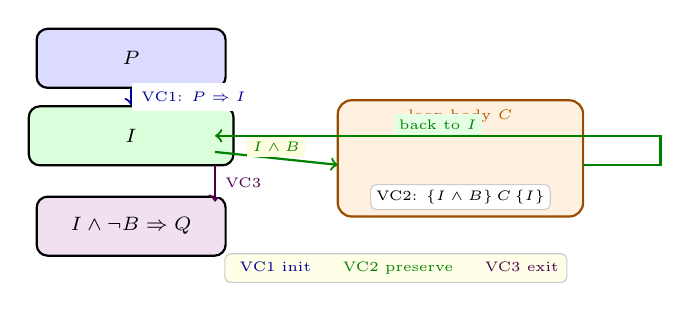
\begin{tikzpicture}[scale=0.82,font=\scriptsize]
\node[draw,fill=blue!14,thick,rounded corners=4pt,minimum width=2.4cm,minimum height=0.75cm] (p) at (0,2.6) {$P$};
\node[draw,fill=green!14,thick,rounded corners=4pt,minimum width=2.6cm,minimum height=0.75cm] (i) at (0,1.4) {$I$};
\draw[->,thick,blue!60!black] (p) -- (i) node[midway,right,font=\tiny,fill=white] {VC1: $P\Rightarrow I$};
\draw[fill=orange!12,draw=orange!60!black,thick,rounded corners=5pt] (3.2,0.15) rectangle (7.0,1.95);
\node[font=\tiny,orange!70!black] at (5.10,1.70) {loop body $C$};
\draw[->,thick,green!50!black] (1.3,1.15) -- (3.2,0.95) node[midway,above,font=\tiny,fill=yellow!12,inner sep=2pt] {$I\land B$};
\draw[->,thick,green!50!black] (7.0,0.95) -- (8.2,0.95) -- (8.2,1.40) -- (1.3,1.40) node[midway,above,font=\tiny,fill=green!10,inner sep=2pt] {back to $I$};
\node[font=\tiny,fill=white,draw=gray!40,rounded corners=2pt,inner sep=2pt] at (5.10,0.45) {VC2: $\{I\land B\}\,C\,\{I\}$};
\node[draw,fill=violet!12,thick,rounded corners=4pt,minimum width=2.4cm,minimum height=0.75cm] (q) at (0,0.0) {$I\land\neg B\Rightarrow Q$};
\draw[->,thick,violet!60!black] (1.30,0.95) -- (1.30,0.38) node[midway,right,font=\tiny,fill=white] {VC3};
\node[font=\tiny,align=left,fill=yellow!10,draw=gray!40,rounded corners=2pt,inner sep=3pt] at (4.1,-0.65) {\textcolor{blue!60!black}{$\blacksquare$ VC1 init} \quad \textcolor{green!50!black}{$\blacksquare$ VC2 preserve} \quad \textcolor{violet!60!black}{$\blacksquare$ VC3 exit}};
\end{tikzpicture}
\caption{The three VCs of the while-rule: enter inside $I$, stay inside each lap, and exit into $Q$. If all three hold, the loop is partially correct.}
\label{fig:three-vcs}
\end{figure}

\begin{figure}[h]\centering
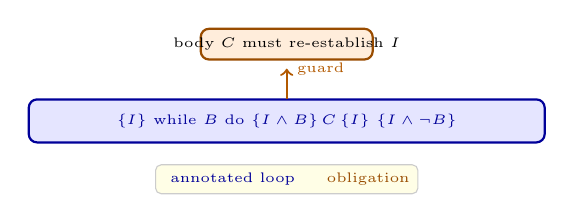
\begin{tikzpicture}[scale=0.78,font=\scriptsize]
\draw[fill=blue!10,draw=blue!60!black,thick,rounded corners=3pt] (0,0) rectangle (8.4,0.70);
\node[font=\tiny,blue!60!black] at (4.2,0.35) {$\{I\}$ while $B$ do $\{I\land B\}\,C\,\{I\}$ $\{I\land\neg B\}$};
\draw[->,thick,orange!70!black] (4.2,0.70) -- (4.2,1.20) node[right,font=\tiny] {guard};
\draw[fill=orange!14,draw=orange!60!black,thick,rounded corners=3pt] (2.8,1.35) rectangle (5.6,1.85);
\node[font=\tiny] at (4.2,1.60) {body $C$ must re-establish $I$};
\node[font=\tiny,align=left,fill=yellow!10,draw=gray!40,rounded corners=2pt,inner sep=3pt] at (4.2,-0.60) {\textcolor{blue!60!black}{$\blacksquare$ annotated loop} \quad \textcolor{orange!60!black}{$\blacksquare$ obligation}};
\end{tikzpicture}
\caption{Annotated loop: the invariant appears explicitly as $\{I\}$ at the head; the body proof may assume $I\land B$ and must show $I$.}
\label{fig:annotated-loop}
\end{figure}

% ============================================================
\section{Warm-Up: Summation Revisited as a VC Proof}
\label{sec:sum-vc}
Program $S\equiv s:=0;\;i:=0;\;\texttt{while }i<n\texttt{ do }(s:=s+a[i];\,i:=i+1)$ with spec $\{n\ge0\}\,S\,\{s=\sum_{j=0}^{n-1}a[j]\}$.

Pick $I\equiv 0\le i\le n\land s=\sum_{j=0}^{i-1}a[j]$ (Chapter~3). VCs:

\textbf{VC1:} $n\ge0\land s=0\land i=0 \Rightarrow I$ holds (empty sum).

\textbf{VC2:} $\{I\land i<n\}\,s:=s+a[i];\,i:=i+1\,\{I\}$. After assignments, $s'=\sum_{j=0}^{i-1}a[j]+a[i]=\sum_{j=0}^{i}a[j]$ and $i'=i+1$, so $s'=\sum_{j=0}^{i'-1}a[j]$.

\textbf{VC3:} $I\land i\ge n\Rightarrow i=n\Rightarrow s=\sum_{j=0}^{n-1}a[j]$.

All three are pure arithmetic—no program reasoning remains. That is the point: VCs are logic formulas an SMT solver can discharge. The human contribution ends at $I$; the solver handles the rest by unfolding definitions.

\begin{remark}[Automation boundary]
Writing $I$ is the \emph{specification} task; discharging VCs is the \emph{verification} task. Tools like Dafny ask you for the former and automate the latter. Hence learning to craft $I$ is not automatable away—it is the core intellectual skill of this course.
\end{remark}

\begin{lstlisting}[language=Python, caption={VCs as Python assertions: each VC is a logical check, not a test of runs.}, label={lst:vc-py}]
# VC1: initiation
def vc1(n,s,i): return not (n>=0 and s==0 and i==0) or (0<=i<=n and s==sum([]))
# VC2: preservation (encoded as wp of body, Ch 7)
def vc2_body(a,i,s,n):
    # assume I and i<n; after s+=a[i]; i+=1, does I hold?
    I_before = (0<=i<=n and s==sum(a[0:i]))
    if not (I_before and i<n): return True
    s2, i2 = s+a[i], i+1
    return 0<=i2<=n and s2==sum(a[0:i2])
# VC3: exit
def vc3(a,s,i,n):
    I = (0<=i<=n and s==sum(a[0:i]))
    return not (I and not (i<n)) or (s==sum(a))
\end{lstlisting}

% ============================================================
\section{Search and Euclid: Invariants That Carry Quantifiers}
\label{sec:search-euclid}
\textbf{Linear search:} $i:=0;\texttt{while }i<n\land a[i]\neq key\texttt{ do }i:=i+1$ with post $(i=n\Rightarrow\forall j<n.\,a[j]\neq key)\land(i<n\Rightarrow a[i]=key)$. Invariant: $I\equiv 0\le i\le n\land\forall j<i.\,a[j]\neq key$. VC2 uses the fact that if $\forall j<i.\,a[j]\neq key$ and $a[i]\neq key$ then $\forall j<i+1.\,a[j]\neq key$.

\textbf{Euclid GCD:} $a,b>0;\;\texttt{while }a\neq b\texttt{ do if }a>b\texttt{ then }a:=a-b\texttt{ else }b:=b-a$ with post $a=\gcd(a_0,b_0)$ where $a_0,b_0$ are initial values (ghost variables). Invariant: $I\equiv a>0\land b>0\land \gcd(a,b)=\gcd(a_0,b_0)$. Preservation uses $\gcd(a-b,b)=\gcd(a,b)$ when $a>b$. Exit $a=b$ gives $a=\gcd(a_0,b_0)$.

\begin{figure}[h]\centering
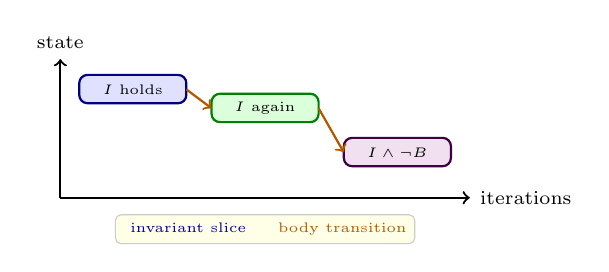
\begin{tikzpicture}[scale=0.80,font=\scriptsize]
\draw[->,thick] (0,0) -- (6.5,0) node[right] {iterations};
\draw[->,thick] (0,0) -- (0,2.2) node[above] {state};
\draw[fill=blue!12,draw=blue!50!black,thick,rounded corners=3pt] (0.3,1.50) rectangle (2.0,1.95);
\node[font=\tiny] at (1.15,1.72) {$I$ holds};
\draw[fill=green!14,draw=green!50!black,thick,rounded corners=3pt] (2.4,1.20) rectangle (4.1,1.65);
\node[font=\tiny] at (3.25,1.42) {$I$ again};
\draw[fill=violet!12,draw=violet!50!black,thick,rounded corners=3pt] (4.5,0.50) rectangle (6.2,0.95);
\node[font=\tiny] at (5.35,0.72) {$I\land\neg B$};
\draw[->,thick,orange!70!black] (2.0,1.72) -- (2.4,1.42);
\draw[->,thick,orange!70!black] (4.1,1.42) -- (4.5,0.72);
\node[font=\tiny,align=left,fill=yellow!10,draw=gray!40,rounded corners=2pt,inner sep=3pt] at (3.25,-0.50) {\textcolor{blue!60!black}{$\blacksquare$ invariant slice} \quad \textcolor{orange!70!black}{$\blacksquare$ body transition}};
\end{tikzpicture}
\caption{Euclid trace: each iteration preserves $I\equiv\gcd(a,b)=\gcd(a_0,b_0)$; exit with $a=b$ forces the post. The invariant is a coloured bar that never changes height.}
\label{fig:euclid-trace}
\end{figure}

\begin{lstlisting}[language=Python, caption={Euclid with ghost variables to state the invariant: $a_0,b_0$ never change but appear in $I$.}, label={lst:euclid-py}]
def gcd_verify(a,b):
    a0,b0 = a,b
    # I: a>0 and b>0 and gcd(a,b)==gcd(a0,b0)
    import math
    assert a>0 and b>0 and math.gcd(a,b)==math.gcd(a0,b0)
    while a != b:
        if a > b: a = a - b
        else:     b = b - a
        assert a>0 and b>0 and math.gcd(a,b)==math.gcd(a0,b0)
    assert a == math.gcd(a0,b0)  # I and not B => post
    return a
\end{lstlisting}

% ============================================================
\section{Nested Loops and Auxiliary Variables}
\label{sec:nested}
Nested loops conjoin invariants: outer $I_{out}$ and inner $I_{in}$ with $I_{out}$ preserved across the whole inner loop as if it were one command. Example: sum of matrix $m\times n$: outer $i$ has $I_{out}\equiv \sum_{\text{rows }<i}$, inner $j$ has $I_{in}\equiv I_{out}\land \sum_{\text{cols }<j\text{ in row }i}$. Inner exit re-establishes $I_{out}$ for next outer iteration.

Sometimes $I$ needs an \emph{auxiliary (ghost) variable} not in the program to remember history. For GCD we used $a_0,b_0$; for ``$x$ is the number of times $B$ was true'' we add counter $t$ that shadows the loop. Auxiliary variables are removed before execution—they are proof scaffolding.

% ============================================================
\section{Generating VCs Mechanically}
\label{sec:vc-gen}
Given annotated program, VC generation is syntax-directed: walk the tree, emit implications. For sequence $C_1;C_2$, compose VCs; for conditional, split on guard; for while, emit the three VCs above. Tools like Why3 do this and feed formulas to Z3/CVC5. Your job as human: supply $I$; the rest is automatic.

\begin{remark}[Annotation burden]
The only creative input is the invariant. Everything else—assignment axiom $Q[x\mapsto e]$, sequence, conditional, consequence—is deterministic. This is why loop verification is ``find $I$, then win''.
\end{remark}

% ============================================================
\section{Case Study: Verifying Partition}
\label{sec:partition}
Partition (Lomuto) $i:=-1;\;\texttt{for }j=0\texttt{ to }n-1\texttt{ do if }a[j]\le pivot\texttt{ then }i:=i+1;\,swap(a[i],a[j])$ with post $a[0..i]\le pivot < a[i+1..n-1]$. Loop invariant after $j$ iterations:
\[
I\equiv -1\le i<j\le n\ \land\ (\forall k\le i.\,a[k]\le pivot)\ \land\ (\forall k.\,i<k<j\Rightarrow a[k]>pivot).
\]
VC2 splits on $a[j]\le pivot$: when true, incrementing $i$ and swapping preserves both quantifier blocks; when false, $j$ advances while $i$ stays, and the second block extends by one. VC3 with $j=n$ yields the desired post: all elements classified. This is exactly the invariant that makes quicksort's correctness routine.

The three-region picture helps: everything left of $i$ is $\le pivot$ (green), between $i+1$ and $j-1$ is $>pivot$ (red), and $j$ onward is unprocessed (grey). Each iteration moves $j$ right by one and, if needed, expands the green region. The invariant is that the coloured prefix is always correctly classified.

\begin{example}[Pitfall: off-by-one invariant]
If you write $I$ as $0\le i\le n$ for partition where $i$ starts at $-1$, VC1 fails ($i=-1\not\ge0$) and you chase a phantom bug. Bounds in $I$ must match initialization. Always test VC1 on the actual initial values before proving VC2.
\end{example}

\begin{remark}[Inner vs outer]
For nested loops the inner invariant may temporarily break the outer one mid-iteration, but must restore it by inner exit. Think of pushing a stack: inner completes, then outer's ``rows done'' advances by one. If inner invariant does not imply outer's preservation, composition fails.
\end{remark}

% ============================================================
\section{Exercises}
\label{sec:ch04-exercises}
\begin{enumerate}[label=E4.\arabic*, leftmargin=*, itemsep=0.6em]
    \item \textbf{VCs for summation.} Write VC1--3 for $s:=0;\,i:=0;\,\texttt{while }i<n\texttt{ do }s:=s+a[i];\,i:=i+1$ with $I\equiv0\le i\le n\land s=\sum_{j<i}a[j]$ as formal implications.
    \item \textbf{Search preservation.} Prove VC2 for linear search: assuming $\forall j<i.\,a[j]\neq key$ and $a[i]\neq key$, show $\forall j<i+1.\,a[j]\neq key$.
    \item \textbf{Euclid exit.} From $I\equiv\gcd(a,b)=\gcd(a_0,b_0)$ and $\neg(a\neq b)$, derive $a=\gcd(a_0,b_0)$.
    \item \textbf{Nested sum.} Give $I_{out}$ and $I_{in}$ for summing an $m\times n$ matrix row-major. Explain why $I_{in}$ must mention $I_{out}$.
    \item \textbf{Auxiliary need.} Show a program counting iterations where post mentions ``number of iterations'' cannot be proved without an auxiliary counter. Propose it and state its invariant.
\end{enumerate}

\section*{Chapter Notes}
Verification conditions originate with Floyd and King. The three-VC presentation is standard in Winskel and Nielson--Nielson. Gries gives many loop invariants; Kaldewaij's \emph{Programming: The Derivation of Algorithms} is a rich source of nested-loop examples.

\smallskip
\begin{remark}[Workflow]
When stuck, write the post $Q$ first, then derive $I$ as ``$Q$ with $n$ replaced by $i$ plus bounds''. For summation $Q$ is sum to $n$, so $I$ is sum to $i$; for search $Q$ is $\forall j<n$, so $I$ is $\forall j<i$. This syntactic shadowing heuristic invents $I$ for many standard loops.
\end{remark}

\smallskip
% Keep air: verification is iterative
% End of Chapter 4
